\section{Pointing accuracy}
\label{se:pointing}
% + RTA pointing estimate method
% + pointing model
% + pointing error (scan-to-scan scattering)

\begin{figure}[p]
\begin{center}
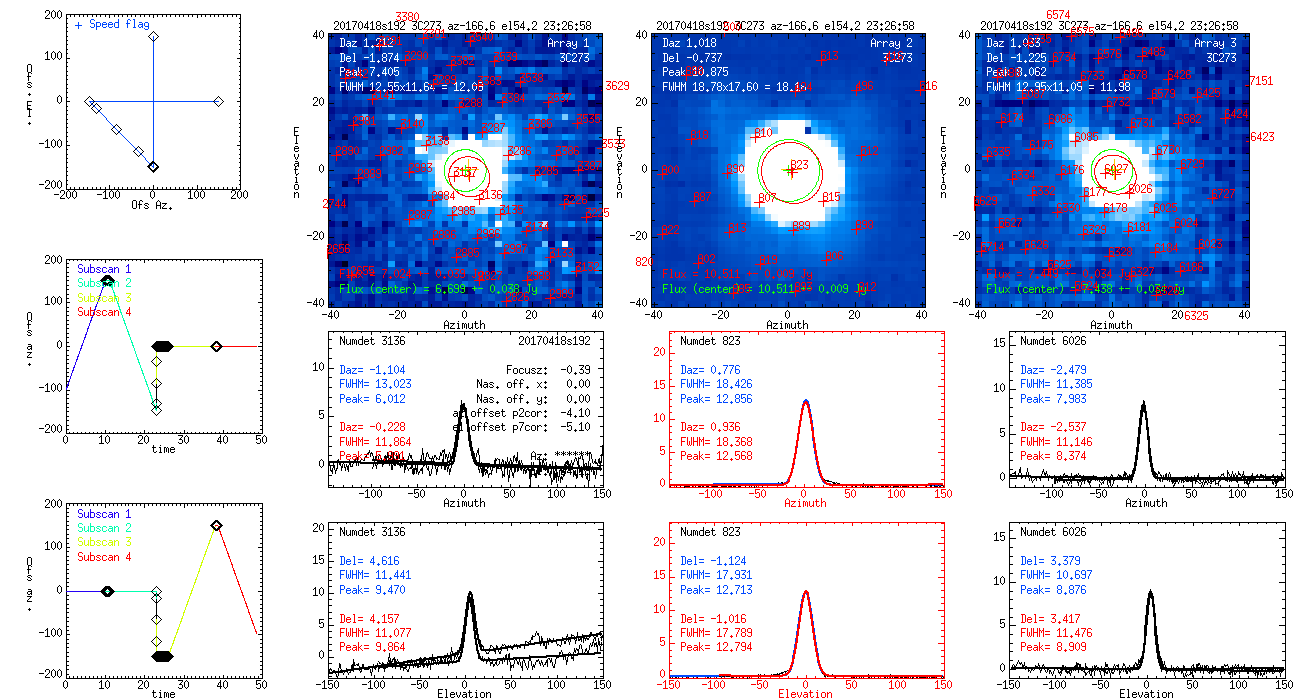
\includegraphics[clip, angle=0, scale = 0.30]{Figures/plot_20170418s192.png}
\caption{Summary plots of the reduction of pointing scan. There is one combined
  map per array to check the overall quality of the scan, and a set of azimuth
  and elevation profiles for one reference detector per array. The 2-mm reference
  detector, highlighed in red, is the the pointing reference detector of
  NIKA2. The location of the peak in azimuth and elevation, as observed by the
  reference detector gives the pointing offset of the current scan.}
\label{fig:ptg}
\end{center}
%\end{figure}
%\begin{figure}[htp]
\begin{center}
\includegraphics[clip, angle=0, scale = 0.70]{Figures/pointing_stats_N2R9.eps}
\caption{Pointing offsets during Run9 observations, before and after the
  derivation of Nasmyth offsets with a pointing session on Feb.~26th, 2017.}
\label{fig:pointing_stats_n2r9}
\end{center}
\end{figure}

Based on general operating experience at the 30-m telescope, we use the so-called
{\em pointing} or {\em cross} scans to monitor the pointing during observations. The
telescope executes a back and forth scan in azimuth and a back and forth scan in
elevation, centered on the observed source. Looking at the timeline profiles of
the reference detector, we fit gaussian profiles and derive the current pointing
offsets of the system in azimuth and elevation. These offsets can then be passed
to PAKO to recenter the next scan (Fig.~\ref{fig:ptg}).

Such scans and their analyses are also used to improve the pointing model
of NIKA2. A pointing session consists in observing about 30 sources on a wide
range of elevations while monitoring the pointing offsets that are measured for
each observation. These offsets are then passed to the IRAM staff who finds
the pointing model parameters that minimize and symetrize the scattering of
these offsets (cf.~Fig.~\ref{fig:ptg_scattering}).

{\bf FM : add a figure showing the IRAM fit}

Fig.~\ref{fig:pointing_stats_n2r9} shows
the pointing corrections that had to be applied during Run9, before and after
the modification of the Nasmyth offsets. 
%the derivation of the new Nasmyth offsets. 
%\noindent {\bf FM : {\it derivation of the new Nasmyth offsets} ->this is has to be explained}\\




While the absolute values of the
corrections is somewhat arbitrary and set around zero for convenience, the
dispersion of the offsets is the true figure of merit of the pointing
corrections. The distribution of corrections after the corrections (in yellow to
red) is clearly more symmetric and narrower than before. During N2R9 run, the pointing accuracy was
1.62 arcsec rms in azimuth and 1.37 arcsec rms in elevation.


{\bf FM : are these values typical ? other runs ?}\\
